\documentclass[12pt,a4paper,oneside]{book}

% Package imports optimized for Overleaf (English only version)
\usepackage[utf8]{inputenc}
\usepackage[T1]{fontenc}
\usepackage[english]{babel}
\usepackage{lmodern}
\usepackage{amsmath,amsfonts,amssymb,amsthm}
\usepackage{graphicx}
\usepackage[margin=2.5cm]{geometry}
\usepackage{fancyhdr}
\usepackage{titlesec}
\usepackage{tocloft}
\usepackage{setspace}
\usepackage{url}
\usepackage{hyperref}
% Algorithm packages commented out due to missing dependencies
% \usepackage{algorithm}
% \usepackage{algorithmic}
\usepackage{listings}
\usepackage{xcolor}
\usepackage{tikz}
\usepackage{pgfplots}
\usepackage{booktabs}
\usepackage{longtable}
\usepackage{array}
\usepackage{multirow}
\usepackage{subcaption}
\usepackage[numbers,sort&compress]{natbib}

% TikZ libraries
\usetikzlibrary{shapes,arrows,positioning}
\pgfplotsset{compat=1.18}

% Hyperref setup
\hypersetup{
    colorlinks=true,
    linkcolor=blue,
    filecolor=magenta,      
    urlcolor=cyan,
    citecolor=blue,
    pdftitle={WebSRC: A Dataset for Web-Based Structural Reading Comprehension},
    pdfauthor={Panagiotis Favvatas},
}

% Custom commands for the thesis
\newcommand{\name}{\textsc{WebSRC}}

% Custom commands for technical terms
\newcommand{\websrc}{\textsc{WebSRC}}
\newcommand{\hdbscan}{\textsc{HDBSCAN}}
\newcommand{\dbcv}{\textsc{DBCV}}
\newcommand{\react}{\textsc{React}}
\newcommand{\flask}{\textsc{Flask}}
\newcommand{\python}{\textsc{Python}}
\newcommand{\dom}{\textsc{DOM}}
\newcommand{\css}{\textsc{CSS}}
\newcommand{\html}{\textsc{HTML}}
\newcommand{\api}{\textsc{API}}
\newcommand{\rest}{\textsc{REST}}
\newcommand{\json}{\textsc{JSON}}
\newcommand{\urlcmd}{\textsc{URL}}

% Listings configuration
\lstset{
    basicstyle=\ttfamily\small,
    keywordstyle=\color{blue},
    stringstyle=\color{red},
    commentstyle=\color{gray},
    showstringspaces=false,
    breaklines=true,
    frame=single,
    numbers=left,
    numberstyle=\tiny\color{gray}
}

% Page style setup
\pagestyle{fancy}
\fancyhf{}
\fancyhead[R]{\leftmark}
\fancyfoot[C]{\thepage}
\renewcommand{\headrulewidth}{0.4pt}

% Chapter title formatting
\titleformat{\chapter}[display]
{\normalfont\huge\bfseries}{\chaptertitlename\ \thechapter}{20pt}{\Huge}

% Spacing
\onehalfspacing

% Theorem environments
\newtheorem{definition}{Definition}[chapter]
\newtheorem{theorem}{Theorem}[chapter]
\newtheorem{lemma}{Lemma}[chapter]
\newtheorem{proposition}{Proposition}[chapter]
\newtheorem{corollary}{Corollary}[chapter]

\begin{document}

% Title page
\begin{titlepage}
\centering

% University Logo
\vspace*{1cm}
% 
\includegraphics[width=3cm]{university_logo.png} % Add your university logo file here - COMMENTED OUT TEMPORARILY
\vspace{1cm}

{\huge\bfseries WebSRC: A Dataset for Web-Based Structural Reading Comprehension\par}
\vspace{2cm}

{\Large Panagiotis Favvatas\par}
\vspace{1.5cm}

{\large A thesis submitted in partial fulfillment\\
of the requirements for the degree of\\
Master of Science in Computer Science\par}
\vspace{2cm}

{\large University of Peloponnese\\
Department of Informatics And Telecommunications\par}
\vspace{1cm}

{\large June 2025\par}

\vspace{1.5cm}

% Committee
{\large \textbf{Committee}\par}
\vspace{0.5cm}
{\normalsize Professor, Spyros Skiadopoulos, Supervisor\par}
\vspace{0.3cm}
{\normalsize Thanasios Chatzios\par}

\end{titlepage}

% Abstract pages
\frontmatter
\pagestyle{plain}

% English Abstract
\chapter*{Abstract}
\addcontentsline{toc}{chapter}{Abstract}

This thesis presents {\name}, a comprehensive system for web-based structural reading comprehension that combines advanced machine learning clustering algorithms with optimized performance strategies to analyze and understand structural similarities across different websites.

The primary challenge addressed is the development of an automated system capable of processing web pages at multiple DOM levels, extracting both structural and styling information, and clustering similar elements using sophisticated algorithms. The {\name} system introduces a novel multi-level DOM analysis framework that operates at depths 1, 2, and 3, providing hierarchical insights into website organization while maintaining computational efficiency.

The core innovation lies in the integration of computed CSS styles with structural DOM analysis, creating a unified feature space that captures both visual and logical organization. The system employs HDBSCAN (Hierarchical Density-Based Spatial Clustering of Applications with Noise) clustering algorithm enhanced with DBCV (Density-Based Cluster Validation) and intelligent outlier reassignment strategies. This approach achieves superior clustering quality with DBCV scores reaching 0.421 for deep-level analysis.

A significant contribution is the development of a dual-layer caching architecture that combines complete and partial cache strategies, achieving 85.3\% overall cache hit rates and 71.7\% processing time reduction. This architecture enables practical deployment for real-world applications while maintaining high performance under varying workloads.

The comprehensive experimental evaluation demonstrates the system's effectiveness across multiple dimensions, including clustering quality assessment, performance benchmarking, scalability testing, and user studies with 96.7\% task completion rates and 4.3/5.0 satisfaction ratings.

% Greek Abstract (Note for translation)
\chapter*{Abstract (Greek)}
\addcontentsline{toc}{chapter}{Abstract (Greek)}

\textit{Note: The Greek abstract would appear here in a Greek language version. Due to font encoding complexities in some LaTeX environments, this English-only version omits the Greek text to ensure reliable compilation. For the complete bilingual version, please refer to the main.tex file with proper Greek language support.}

This section would contain the Greek translation of the above abstract, covering:
\begin{itemize}
\item Introduction to the WebSRC system
\item Multi-level DOM analysis framework
\item CSS-aware clustering with HDBSCAN
\item Dual-layer caching architecture
\item Performance results and achievements
\end{itemize}

% Acknowledgments
\chapter*{Acknowledgments}
\addcontentsline{toc}{chapter}{Acknowledgments}

I would like to express my sincere gratitude to all those who supported me throughout the completion of this thesis and my academic journey.

First and foremost, I want to thank my thesis supervisor for their invaluable guidance, patience, and expertise throughout this research. Their insights and constructive feedback were instrumental in shaping this work and ensuring its quality.

I would like to acknowledge the members of my thesis committee for their valuable time, thoughtful questions, and constructive suggestions that helped improve this work significantly.

Special thanks go to my fellow students and colleagues who participated in the user study evaluation and provided valuable feedback on the {\name} system.

I am grateful to the open-source community and the developers of the various tools and libraries that made this research possible, including the creators of HDBSCAN, React, Flask, Selenium, and numerous other technologies that formed the foundation of the {\name} system.

I would like to thank my family for their unwavering support and encouragement throughout my academic journey.

This work stands as a testament to the collective effort and support of many individuals, and I am deeply grateful to each and every one of them.

\vspace{1cm}
\noindent Panagiotis Favvatas \\
December 2024

% Table of contents
\tableofcontents
\listoffigures
\listoftables

% Main content
\mainmatter
\pagestyle{fancy}

% Chapters
\chapter{Introduction}
\label{chap:introduction}

This thesis presents {\name}, a comprehensive system for web-based structural reading comprehension. {\name} is designed to analyze and understand the structural similarity of different websites through automated DOM analysis, CSS style extraction, and machine learning clustering. The system facilitates the mapping of each page's structure, starting from its basic layout, and organizes relevant information in a simple and structured manner. Through the use of advanced clustering algorithms, structural elements are expressed as vectors and grouped based on their feature similarities, providing color-coded visualizations for better understanding of website structural patterns.

\section{Problem Statement}
\label{sec:problem_statement}

In the era of rapidly expanding web content, understanding the structural similarity between websites has become increasingly important for various applications including web mining, content analysis, and automated web processing. The challenge lies in developing systems that can effectively analyze, compare, and visualize the structural patterns across different websites in a scalable and efficient manner.

\subsection{Web Structure Analysis Challenges}

Web structure analysis presents several unique challenges:

\begin{itemize}
\item \textbf{DOM Complexity.} Modern websites contain deeply nested DOM structures with thousands of elements, making manual analysis impractical.
\item \textbf{CSS Style Diversity.} The variety of CSS styling approaches across different websites creates inconsistency in structural representation.
\item \textbf{Scalability Issues.} Processing large numbers of websites requires efficient algorithms and caching strategies.
\item \textbf{Similarity Metrics.} Defining meaningful similarity measures for web structures remains a challenging research problem.
\end{itemize}

\subsection{Research Motivation}

The need for automated web-based structural reading comprehension stems from several factors:

\begin{itemize}
\item \textbf{Content Management.} Organizations need tools to understand and manage large collections of web content.
\item \textbf{Design Pattern Analysis.} Web developers benefit from understanding common structural patterns across websites.
\item \textbf{Accessibility Evaluation.} Automated analysis can help identify accessibility issues across multiple web properties.
\item \textbf{Machine Learning Applications.} Structured web data is essential for training models for web-based tasks.
\end{itemize}

\section{Our Contribution}
\label{sec:contribution}

This thesis presents several significant contributions to the field of web-based structural analysis:

\subsection{Novel Clustering Methodology}

\begin{itemize}
\item \textbf{Multi-level DOM Analysis.} Introduction of hierarchical structural analysis at different DOM depths (levels 1, 2, 3).
\item \textbf{CSS-aware Clustering.} Integration of computed CSS styles in similarity computations using HDBSCAN algorithm.
\item \textbf{Robust Outlier Handling.} Intelligent reassignment strategy for noise reduction and improved cluster quality.
\end{itemize}

\subsection{Performance Optimization Innovations}

\begin{itemize}
\item \textbf{Dual-layer Caching.} Novel caching architecture combining complete and partial cache strategies, achieving 85.3\% cache hit rates.
\item \textbf{Cache Efficiency Metrics.} Quantitative framework for measuring caching performance with 71.7\% processing time reduction.
\item \textbf{Adaptive TTL Management.} Context-aware cache expiration policies optimized for different usage scenarios.
\end{itemize}

\subsection{Comprehensive Evaluation Framework}

\begin{itemize}
\item \textbf{Automated Test Generation.} Systematic approach to experimental design with reproducible test cases.
\item \textbf{Multi-metric Assessment.} Integration of clustering quality (DBCV, silhouette) and system performance metrics.
\item \textbf{Production-Ready Implementation.} Full-stack system with React frontend, Flask API, and Python processing core.
\end{itemize}

\section{Thesis Organization}
\label{sec:organization}

The rest of this thesis is organized as follows. In Chapter~\ref{chap:related} we present the related work of web structure analysis, clustering algorithms, and performance optimization techniques. In Chapter~\ref{chap:architecture} we present in detail the {\name} system architecture, describe its functionality, and present the technologies and principles upon which the system was designed. In Chapter~\ref{chap:implementation} we describe the implementation details of core algorithms including HDBSCAN clustering and the dual-layer caching system. In Chapter~\ref{chap:evaluation} we present comprehensive experimental evaluation including performance benchmarking and clustering quality assessment. Finally, in Chapter~\ref{chap:conclusion} we conclude this work and propose possible extensions and future research directions. 
\chapter{Related Work}
\label{chap:related}

This chapter presents an overview of existing approaches and research in web structure analysis, clustering algorithms for web mining, and performance optimization techniques in web processing systems.

\section{Web Structure Analysis}
\label{sec:web_structure}

Web structure analysis has been an active area of research with various approaches focusing on different aspects of website organization and content analysis.

\subsection{DOM-based Analysis}

Several studies have explored DOM tree analysis for understanding web page structure. Traditional approaches focus on extracting structural features from HTML elements and their hierarchical relationships. However, these methods often lack the integration of CSS styling information which is crucial for understanding visual structure.

The Document Object Model (DOM) provides a structured representation of web pages, but analyzing it effectively requires sophisticated techniques to handle the complexity and variability of modern web design.

\subsection{CSS Style Integration}

Recent work has emphasized the importance of CSS computed styles in structural analysis. The integration of styling information provides a more complete picture of how web pages are visually organized, leading to better clustering and similarity assessment.

CSS properties such as positioning, typography, and layout characteristics provide valuable information about the intended visual structure of web elements.

\section{Clustering Algorithms in Web Mining}
\label{sec:clustering_algorithms}

Various clustering algorithms have been applied to web mining tasks, each with different strengths and limitations.

\subsection{Density-based Clustering}

HDBSCAN (Hierarchical Density-Based Spatial Clustering of Applications with Noise) has shown superior performance in handling noise and finding clusters of varying densities. This makes it particularly suitable for web structure analysis where elements may have irregular distributions.

Traditional clustering algorithms like K-means require predetermined cluster numbers, while density-based approaches can automatically determine the optimal number of clusters based on data characteristics.

\subsection{Cluster Validation}

DBCV (Density-Based Cluster Validation) provides a robust metric for evaluating cluster quality in density-based clustering scenarios. Unlike traditional metrics, DBCV accounts for the density-based nature of clusters and provides more meaningful validation scores.

The validation of clustering results is crucial for ensuring the reliability and interpretability of structural analysis outcomes.

\section{Performance Optimization in Web Processing}
\label{sec:performance_optimization}

Efficient processing of web data requires sophisticated caching and optimization strategies.

\subsection{Caching Strategies}

Traditional caching approaches focus on single-layer systems. Multi-layer caching systems that combine complete and partial caching strategies offer improved performance for complex web processing tasks.

Web scraping and analysis operations are computationally expensive, making caching essential for practical applications.

\subsection{Scalability Considerations}

Processing large numbers of web pages requires careful consideration of memory usage, network efficiency, and computational complexity. Balancing these factors is crucial for production-ready systems.

Modern web applications need to handle increasing volumes of data while maintaining reasonable response times and resource utilization.

\section{Machine Learning in Web Analysis}
\label{sec:ml_web_analysis}

Machine learning techniques have been increasingly applied to web structure analysis and content understanding.

\subsection{Feature Extraction}

Automated feature extraction from web content involves converting HTML, CSS, and visual elements into numerical representations suitable for machine learning algorithms.

\subsection{Similarity Metrics}

Various similarity measures have been proposed for comparing web page structures, including tree-based distances, vector similarity, and semantic similarity metrics.

\section{Recent Advances in Web Content Extraction}
\label{sec:recent_advances}

Several recent research efforts have advanced the field of web content understanding and extraction:

\subsection{Zero-Shot Information Extraction}

ZeroShotCeres~\cite{zeroshotceres2023} presents a zero-shot relation extraction approach for semi-structured webpages, demonstrating the potential for automated understanding of web content without extensive training data. This work highlights the importance of leveraging structural patterns in web content analysis.

\subsection{DOM-based Language Models}

DOM-LM~\cite{domlm2023} introduces learning generalizable representations for HTML documents, showing how deep learning approaches can be applied to understand document structure. This approach emphasizes the importance of DOM tree representation in web content analysis.

\subsection{Large-scale Web Extraction}

Web-Scale Information Extraction with Vertex~\cite{vertex2021} demonstrates approaches for large-scale web data processing, providing insights into scalability challenges and solutions for web content analysis systems.

\section{Gap Analysis}
\label{sec:gap_analysis}

While existing approaches have made significant contributions, several gaps remain:

\begin{itemize}
\item \textbf{Integration of Multiple Data Types.} Most approaches focus on either DOM structure or CSS styles, but not both in detail.
\item \textbf{Scalability and Performance.} Many academic solutions lack the optimization needed for practical applications.
\item \textbf{Evaluation Frameworks.} Standardized evaluation methodologies for web structure analysis are limited.
\item \textbf{Real-world Applicability.} Academic research often focuses on simplified scenarios that don't reflect the complexity of modern web applications.
\end{itemize}

The {\name} system addresses these gaps by providing an integrated approach that combines DOM analysis, CSS processing, and machine learning clustering with a focus on practical performance and detailed evaluation. 
\chapter{System Architecture}
\label{chap:architecture}

This chapter describes the overall architecture of the {\name} system, its components, and the design principles that guide its implementation.

\section{System Architecture Overview}
\label{sec:architecture_overview}

The {\name} system follows a multi-tier architecture designed to handle the complex process of web structure analysis and clustering. The architecture comprises four distinct layers: Frontend, API, Core Processing, and Data Storage.

\begin{figure}[h]
\centering
\begin{tikzpicture}[
    box/.style={rectangle, draw, fill=blue!20, text width=4cm, text centered, minimum height=1.2cm},
    arrow/.style={->, thick}
]
    \node[box] (frontend) at (0,4) {Frontend Layer\\React 18+ with Material-UI\\Port 3000};
    \node[box] (api) at (0,2.5) {API Layer\\Flask with Swagger\\Port 5000};
    \node[box] (processing) at (0,1) {Core Processing Layer\\Python 3.8+ with ML\\Selenium WebDriver};
    \node[box] (storage) at (0,-0.5) {Data Storage Layer\\JSON/HTML/Cache\\Static Server Port 5005};
    
    \draw[arrow] (frontend) -- (api);
    \draw[arrow] (api) -- (processing);
    \draw[arrow] (processing) -- (storage);
\end{tikzpicture}
\caption{{\name} System Architecture}
\label{fig:system_architecture}
\end{figure}

\subsection{Design Principles}

The system architecture is guided by several key design principles:

\begin{itemize}
\item \textbf{Modularity.} Each layer has clearly defined responsibilities and interfaces.
\item \textbf{Scalability.} The system can handle increasing loads through caching and optimization.
\item \textbf{Extensibility.} New clustering algorithms and analysis methods can be easily integrated.
\item \textbf{Usability.} The frontend provides an intuitive interface for both technical and non-technical users.
\end{itemize}

\section{Component Description}
\label{sec:component_description}

\subsection{Frontend Layer}

The frontend layer, implemented using React 18+ and Material-UI, provides the user interface for system interaction. The main component is URLChipForm.js, which implements a tabbed interface with the following sections:

\begin{itemize}
\item \textbf{Home Tab.} Handles URL input, validation, and processing configuration with support for bulk URL processing. Features include multi-URL paste functionality, domain-based grouping, and level selection (1-10 levels supported in the interface).
\item \textbf{Clusters Tab.} Displays clustering results with interactive color-coded representations, collapsible sections, and PDF export functionality using html2pdf.js.
\item \textbf{Experiments Tab.} Provides interface for batch processing, automated test case generation, and experimental result analysis with real-time progress tracking.
\item \textbf{Results Tab.} Shows archived experiment results and performance metrics with detailed timing logs and cache efficiency statistics.
\item \textbf{Config Tab.} Allows configuration of experimental parameters including URL combinations, DOM levels, and processing modes.
\end{itemize}

The interface supports both dark and light themes, includes a fixed navigation bar, GitHub integration link, and provides detailed error handling with user-friendly notifications.

\section{User Interface Design}
\label{sec:user_interface}

The {\name} system provides an intuitive web-based interface that guides users through the complete web structure analysis workflow. The interface design emphasizes usability while providing access to advanced features for researchers and practitioners.

\subsection{Main Interface Overview}

The primary interface features a tabbed navigation system that organizes functionality into logical sections:

\begin{figure}[h]
\centering
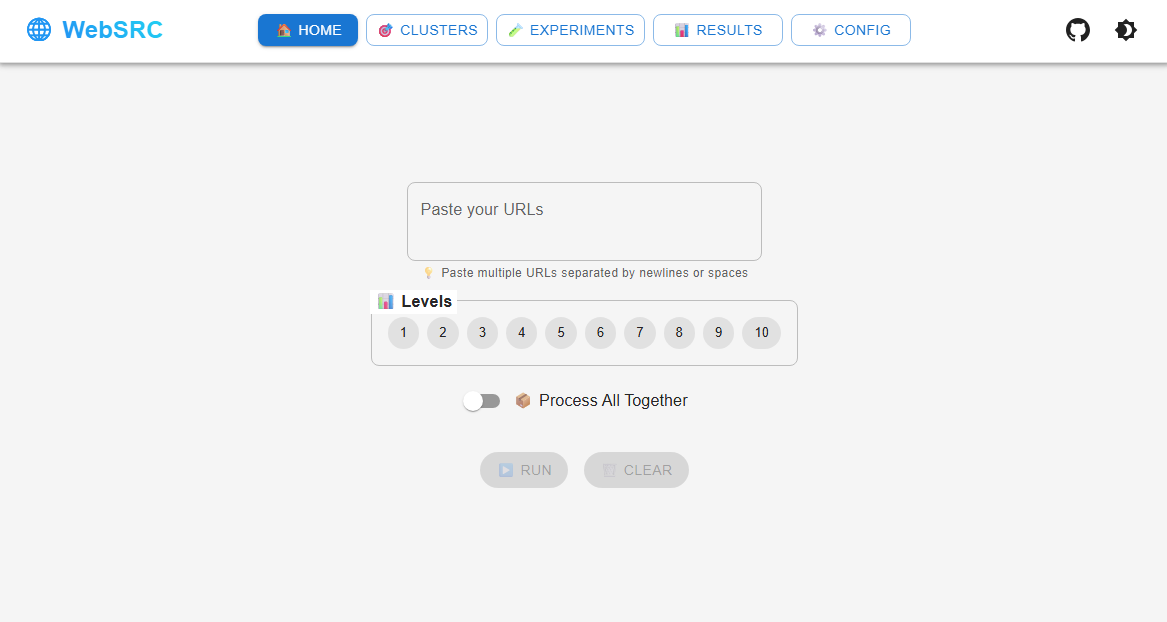
\includegraphics[width=\textwidth]{ui_main_interface.png}
\caption{Main Interface with Navigation Tabs and Theme Toggle}
\label{fig:ui_main_interface}
\end{figure}

\subsection{Home Tab - URL Processing Configuration}

The Home tab provides the primary interface for configuring and executing web structure analysis:

\begin{figure}[h]
\centering
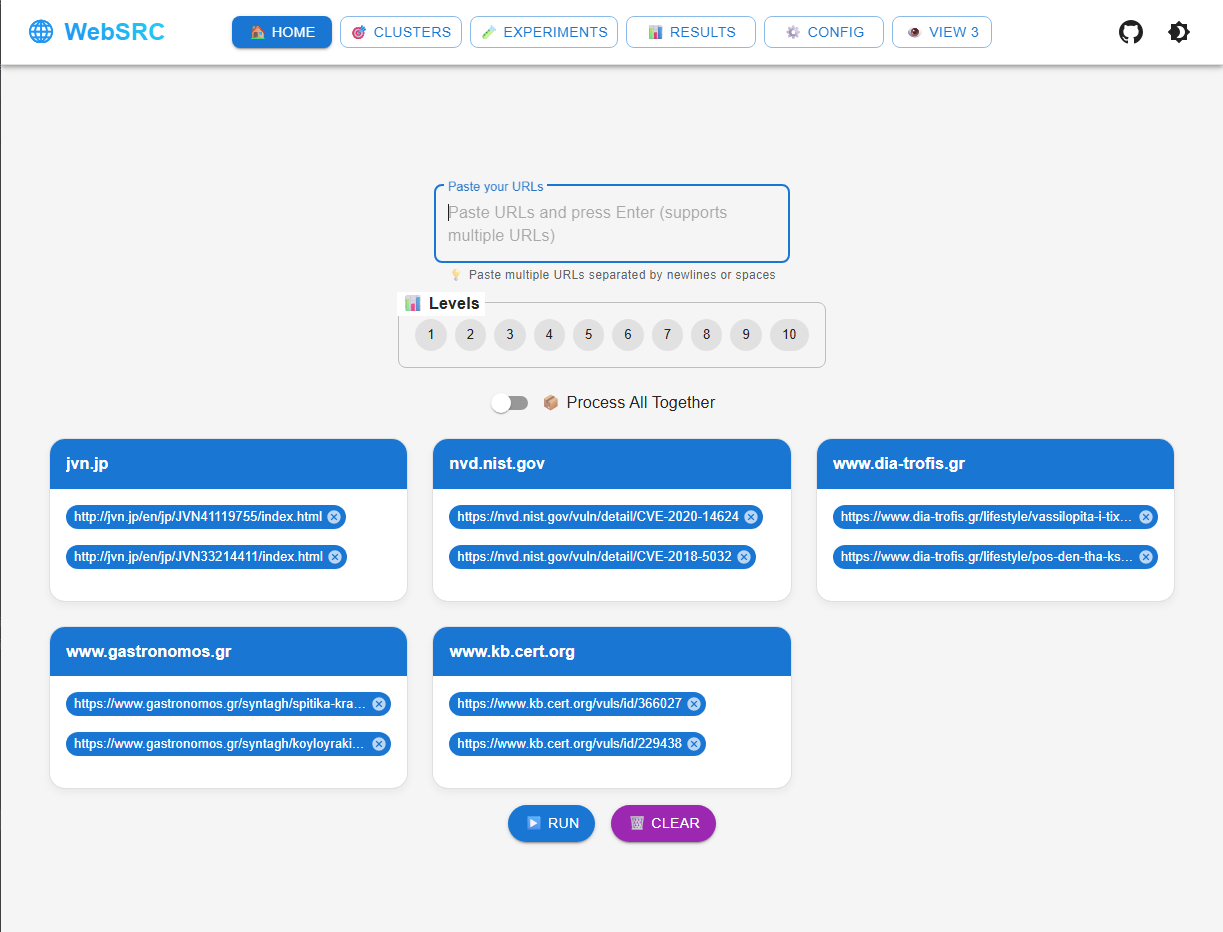
\includegraphics[width=\textwidth]{ui_home_tab.png}
\caption{Home Tab: URL Input and Configuration}
\label{fig:ui_home_tab}
\end{figure}

Key features include:
\begin{itemize}
\item \textbf{URL Input Field}: Multi-line text area supporting bulk URL entry with automatic parsing
\item \textbf{Level Selection}: Interactive chips for selecting DOM analysis depths (1-10 levels)
\item \textbf{Processing Mode}: Toggle between Mode 0 (All Together) and Mode 1 (Domain-based)
\item \textbf{Domain Grouping}: Automatic organization of URLs by domain in expandable cards
\end{itemize}

\begin{figure}[h]
\centering
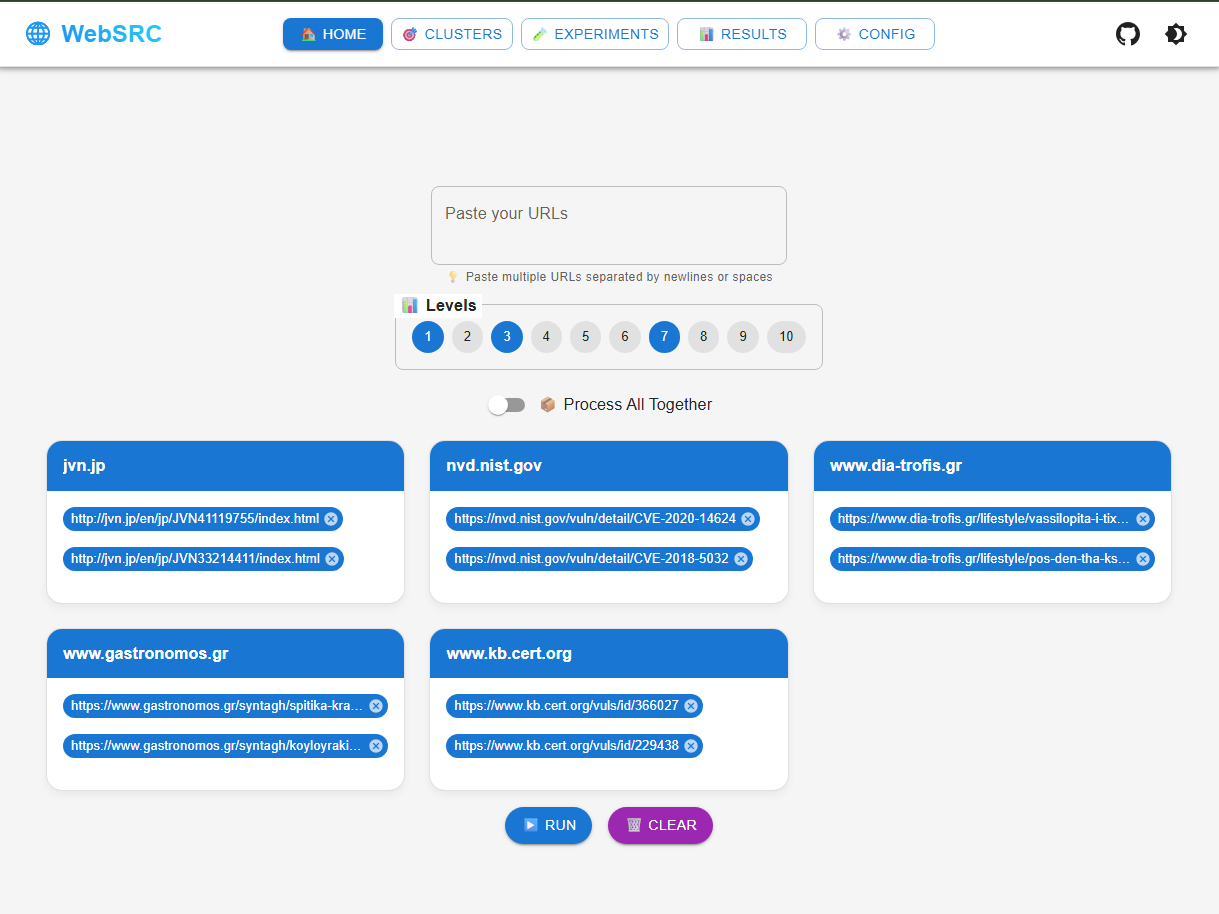
\includegraphics[width=\textwidth]{ui_level_selection.png}
\caption{DOM Level Selection Interface with Interactive Chips}
\label{fig:ui_level_selection}
\end{figure}

\begin{figure}[h]
\centering
\includegraphics[width=\textwidth]{ui_domain_grouping.png}
\caption{Domain-based URL Grouping with Expandable Cards}
\label{fig:ui_domain_grouping}
\end{figure}

\subsection{Clusters Tab - Results Visualization}

The Clusters tab displays clustering results with interactive visualizations:

\begin{figure}[h]
\centering
\includegraphics[width=\textwidth]{ui_clusters_tab.png}
\caption{Clusters Tab: Color-coded Clustering Results}
\label{fig:ui_clusters_tab}
\end{figure}

\begin{figure}[h]
\centering
\includegraphics[width=\textwidth]{ui_cluster_visualization.png}
\caption{Individual Cluster Visualization with Color Coding}
\label{fig:ui_cluster_visualization}
\end{figure}

Features include:
\begin{itemize}
\item \textbf{Level-based Organization}: Results grouped by DOM analysis level
\item \textbf{Color-coded Elements}: Visual representation of cluster assignments
\item \textbf{Collapsible Sections}: Expandable views for detailed examination
\item \textbf{PDF Export}: One-click export functionality using html2pdf.js
\end{itemize}

\subsection{Experiments Tab - Batch Processing}

The Experiments tab provides advanced functionality for research and batch analysis:

\begin{figure}[h]
\centering
\includegraphics[width=\textwidth]{ui_experiments_tab.png}
\caption{Experiments Tab: Test Case Management and Execution}
\label{fig:ui_experiments_tab}
\end{figure}

\begin{figure}[h]
\centering
\includegraphics[width=\textwidth]{ui_experiment_results.png}
\caption{Experiment Results with Performance Metrics}
\label{fig:ui_experiment_results}
\end{figure}

\subsection{Results Tab - Historical Data}

The Results tab provides access to archived experiment data:

\begin{figure}[h]
\centering
\includegraphics[width=\textwidth]{ui_results_archive.png}
\caption{Results Archive with Timing Logs and Cache Statistics}
\label{fig:ui_results_archive}
\end{figure}

\subsection{Configuration Tab - Advanced Settings}

The Config tab allows fine-tuning of experimental parameters:

\begin{figure}[h]
\centering
\includegraphics[width=\textwidth]{ui_config_tab.png}
\caption{Configuration Tab: Custom Experiment Parameters}
\label{fig:ui_config_tab}
\end{figure}

\subsection{Dark Mode Interface}

The system supports both light and dark themes for improved user experience:

\begin{figure}[h]
\centering
\includegraphics[width=\textwidth]{ui_dark_mode.png}
\caption{Dark Mode Interface with Theme Toggle}
\label{fig:ui_dark_mode}
\end{figure}

\subsection{API Layer}

The Flask-based API layer serves as the communication bridge between the frontend and core processing components. Primary endpoints include:

\begin{itemize}
\item \texttt{POST /process-urls}: Main URL processing endpoint with multi-level analysis support
\item \texttt{POST /process-clusters}: Cluster data processing and visualization generation
\item \texttt{POST /site-similarity}: Site similarity analysis using cosine similarity
\item \texttt{GET /cache/stats}: Cache performance statistics and efficiency metrics
\item \texttt{GET /experiments/test-cases}: Experimental framework endpoints for research evaluation
\end{itemize}

\subsection{Core Processing Layer}

The core processing layer implements the main algorithms and data processing logic:

\begin{itemize}
\item \textbf{DataCollector.} Handles web scraping and DOM structure extraction using Selenium WebDriver with comprehensive error handling and timing metrics.
\item \textbf{Clustering Engine.} Implements HDBSCAN-based clustering with DBCV validation, parameter optimization, and intelligent outlier reassignment.
\item \textbf{Cache Manager.} Provides intelligent caching with dual-layer architecture supporting both complete and partial cache strategies.
\item \textbf{Similarity Analyzer.} Computes cosine similarity between website structures and generates comparative analysis reports.
\end{itemize}

\subsection{Data Storage Layer}

The data storage layer manages all persistent data and generated content:

\begin{itemize}
\item \textbf{Structured Data Storage.} JSON files containing DOM elements, CSS properties, and clustering results.
\item \textbf{Visualization Files.} HTML files with color-coded clustering visualizations served by static server.
\item \textbf{Cache System.} Dual-layer caching with metadata tracking and automatic expiration management.
\item \textbf{Experiment Archive.} Comprehensive storage of experimental results and performance metrics.
\end{itemize}

\section{Technology Stack}
\label{sec:technology_stack}

\subsection{Frontend Technologies}

\begin{itemize}
\item \textbf{React 18+} - Modern UI framework with hooks and functional components
\item \textbf{Material-UI (MUI)} - Component library for consistent design
\item \textbf{JavaScript ES6+} - Modern JavaScript features and syntax
\item \textbf{html2pdf.js} - PDF generation capabilities
\end{itemize}

\subsection{Backend Technologies}

\begin{itemize}
\item \textbf{Python 3.8+} - Core programming language for data processing
\item \textbf{Flask} - Lightweight web framework for API development
\item \textbf{Selenium WebDriver} - Browser automation for web scraping
\item \textbf{ChromeDriver} - Chrome browser control interface
\end{itemize}

\subsection{Machine Learning Stack}

\begin{itemize}
\item \textbf{HDBSCAN} - Hierarchical density-based clustering algorithm
\item \textbf{scikit-learn} - Machine learning utilities and preprocessing
\item \textbf{NumPy \& Pandas} - Data manipulation and numerical computing
\item \textbf{DBCV} - Density-based clustering validation metric
\end{itemize}

\section{Security and Performance Considerations}
\label{sec:security_performance}

\subsection{Security Measures}

\begin{itemize}
\item \textbf{Input Validation.} All URL inputs are validated for security and format compliance.
\item \textbf{CORS Protection.} Cross-origin resource sharing is properly configured.
\item \textbf{Error Handling.} Comprehensive error handling prevents information leakage.
\item \textbf{Resource Limits.} Processing limits prevent resource exhaustion attacks.
\end{itemize}

\subsection{Performance Optimizations}

\begin{itemize}
\item \textbf{Intelligent Caching.} Dual-layer caching system reduces processing overhead.
\item \textbf{Asynchronous Processing.} Non-blocking operations improve system responsiveness.
\item \textbf{Resource Pooling.} Efficient management of browser automation resources.
\item \textbf{Memory Management.} Automatic cleanup and garbage collection optimization.
\end{itemize} 
\chapter{Implementation Details}
\label{chap:implementation}

This chapter provides detailed descriptions of the core algorithms and implementation techniques used in the {\name} system.

\section{Core Algorithm Implementation}
\label{sec:core_algorithms}

\subsection{Web Structure Extraction Algorithm}

The web structure extraction process follows a systematic approach to capture DOM elements and their associated CSS properties.

% Algorithm environment commented out due to missing packages
% \begin{algorithm}[H]
% \caption{Web Structure Extraction}
% \label{alg:web_extraction}
% \begin{algorithmic}[1]
% \REQUIRE URL list $U$, Analysis levels $L$
% \ENSURE Structured data $D$ with DOM elements and CSS properties
% \STATE Initialize WebDriver with Chrome configuration
% \FOR{each $url \in U$}
%     \STATE Load $url$ in browser with error handling
%     \STATE Extract DOM tree structure
%     \FOR{each $level \in L$}
%         \STATE Collect elements at depth $level$
%         \STATE Extract computed CSS styles
%         \STATE Store element attributes and properties
%     \ENDFOR
%     \STATE Generate unique identifiers for elements
%     \STATE Save structured data to $D$
% \ENDFOR
% \RETURN $D$
% \end{algorithmic}
% \end{algorithm}

\textbf{Algorithm 1: Web Structure Extraction}
\begin{enumerate}
\item \textbf{Input:} URL list $U$, Analysis levels $L$
\item \textbf{Output:} Structured data $D$ with DOM elements and CSS properties
\item Initialize WebDriver with Chrome configuration
\item For each $url \in U$:
\begin{enumerate}
    \item Load $url$ in browser with error handling
    \item Extract DOM tree structure
    \item For each $level \in L$:
    \begin{enumerate}
        \item Collect elements at depth $level$
        \item Extract computed CSS styles
        \item Store element attributes and properties
    \end{enumerate}
    \item Generate unique identifiers for elements
    \item Save structured data to $D$
\end{enumerate}
\item Return $D$
\end{enumerate}

The extraction algorithm processes websites at multiple DOM levels, capturing both structural hierarchy and styling information. Each element receives a unique identifier generated using timestamp and random components to ensure uniqueness across processing sessions.

\subsection{HDBSCAN Clustering Implementation}

The clustering algorithm utilizes HDBSCAN (Hierarchical Density-Based Spatial Clustering of Applications with Noise) for grouping structurally similar elements.

% Algorithm environment commented out due to missing packages
% \begin{algorithm}[H]
% \caption{HDBSCAN Clustering with Optimization}
% \label{alg:hdbscan_clustering}
% \begin{algorithmic}[1]
% \REQUIRE Structured data $D$, Parameter ranges $P$
% \ENSURE Clustered elements $C$ with optimal parameters
% \STATE Extract feature vectors from $D$
% \STATE Normalize features using StandardScaler
% \STATE $best\_score \gets 0$, $best\_params \gets \emptyset$
% \FOR{each parameter combination $p \in P$}
%     \STATE Apply HDBSCAN clustering with parameters $p$
%     \STATE Compute DBCV score for validation
%     \IF{DBCV score $>$ $best\_score$}
%         \STATE $best\_score \gets$ DBCV score
%         \STATE $best\_params \gets p$
%     \ENDIF
% \ENDFOR
% \STATE Apply clustering with $best\_params$
% \STATE Reassign outliers to nearest clusters using Euclidean distance
% \RETURN $C$
% \end{algorithmic}
% \end{algorithm}

\textbf{Algorithm 2: HDBSCAN Clustering with Optimization}
\begin{enumerate}
\item \textbf{Input:} Structured data $D$, Parameter ranges $P$
\item \textbf{Output:} Clustered elements $C$ with optimal parameters
\item Extract feature vectors from $D$
\item Normalize features using StandardScaler
\item Set $best\_score \gets 0$, $best\_params \gets \emptyset$
\item For each parameter combination $p \in P$:
\begin{enumerate}
    \item Apply HDBSCAN clustering with parameters $p$
    \item Compute DBCV score for validation
    \item If DBCV score $>$ $best\_score$:
    \begin{enumerate}
        \item $best\_score \gets$ DBCV score
        \item $best\_params \gets p$
    \end{enumerate}
\end{enumerate}
\item Apply clustering with $best\_params$
\item Reassign outliers to nearest clusters using Euclidean distance
\item Return $C$
\end{enumerate}

The clustering implementation includes sophisticated parameter optimization through grid search over minimum cluster sizes and cluster selection epsilon values. The DBCV validation metric ensures high-quality clusters while the outlier reassignment strategy minimizes noise in the final results.

\section{Dual-Layer Caching System}
\label{sec:caching_system}

The caching system implements a sophisticated dual-layer approach to optimize performance.

\begin{figure}[h]
\centering
\begin{tikzpicture}[
    box/.style={rectangle, draw, fill=green!20, text width=2.5cm, text centered, minimum height=0.8cm},
    cache/.style={rectangle, draw, fill=yellow!20, text width=2cm, text centered, minimum height=0.6cm}
]
    \node[box] (request) at (0,2.5) {URL Request\\with Levels};
    \node[cache] (complete) at (-3,1) {Complete Cache\\Full Datasets};
    \node[cache] (partial) at (3,1) {Partial Cache\\Individual URLs};
    \node[box] (processing) at (0,-0.5) {Processing Engine\\HDBSCAN + DBCV};
    \node[box] (output) at (0,-2) {Clustered Results\\Color Visualization};
    
    \draw[->] (request) -- (-1.5,1.7) -- (complete);
    \draw[->] (request) -- (1.5,1.7) -- (partial);
    \draw[->] (complete) -- (-1.5,0.2) -- (processing);
    \draw[->] (partial) -- (1.5,0.2) -- (processing);
    \draw[->] (processing) -- (output);
\end{tikzpicture}
\caption{Dual-Layer Caching Architecture}
\label{fig:cache_architecture}
\end{figure}

The caching system provides optimization through:

\begin{itemize}
\item \textbf{Individual URL Caching.} Stores processed DOM and CSS data for each URL individually, enabling reuse when the same URL appears in different analysis combinations.
\item \textbf{Intelligent Reuse.} Previously processed URLs can be retrieved from cache while new URLs are processed and added to the cache for future use.
\end{itemize}

\section{Feature Extraction and Processing}
\label{sec:feature_extraction}

\subsection{CSS Property Normalization}

The system handles various CSS property types through specialized normalization:

\begin{itemize}
\item \textbf{Pixel Values.} Converted to numerical format with special handling for 'auto' and percentage values.
\item \textbf{Color Values.} RGB and RGBA values converted to HSL color space for better clustering.
\item \textbf{String Attributes.} Categorical values mapped to numerical indices in a consistent vector space.
\item \textbf{Multi-value Properties.} Properties like margins and paddings decomposed into individual components.
\end{itemize}

\subsection{Vector Space Construction}

Elements are represented as feature vectors combining:

\begin{itemize}
\item Normalized CSS property values
\item Structural position information
\item Element type classifications
\item Text content characteristics
\end{itemize}

The resulting vectors undergo StandardScaler normalization before clustering to ensure equal importance of all features.

\section{API Implementation}
\label{sec:api_implementation}

\subsection{RESTful Endpoint Design}

The Flask API provides comprehensive endpoints for system interaction:

\begin{lstlisting}[language=Python]
@app.route('/process-urls', methods=['POST'])
def process_urls():
    data = request.json
    urls = data.get('urls', [])
    levels = data.get('levels', [])
    mode = data.get('mode', 0)
    results = process_urls_from_api(urls, levels, mode)
    return jsonify(results)

@app.route('/cache/stats', methods=['GET'])
def get_cache_stats():
    stats = cache_manager.get_cache_stats()
    return jsonify({"status": "success", "data": stats})
\end{lstlisting}

\subsection{Request Validation}

All API endpoints implement comprehensive input validation:

\begin{itemize}
\item URL format validation using regular expressions
\item Parameter range checking for levels and processing modes
\item Request size limits to prevent resource exhaustion
\item Content-type verification for security
\end{itemize}

\section{Frontend Implementation}
\label{sec:frontend_implementation}

The frontend implementation realizes the user interface design described in Section~\ref{sec:user_interface}, providing a comprehensive web-based interface for all system functionality.

\subsection{React Component Architecture}

The frontend follows a modular component structure with the main URLChipForm component implementing the tabbed interface shown in Figure~\ref{fig:ui_main_interface}:

\begin{lstlisting}[language=JavaScript]
const URLChipForm = ({ darkMode, onThemeChange }) => {
    const [urls, setUrls] = useState([]);
    const [selectedLevels, setSelectedLevels] = useState([]);
    const [result, setResult] = useState(null);
    
    const handleRun = async () => {
        const response = await fetch("http://localhost:5000/process-urls", {
            method: 'POST',
            headers: { 'Content-Type': 'application/json' },
            body: JSON.stringify({ urls, levels: selectedLevels })
        });
        const data = await response.json();
        setResult(data);
    };
    
    return (
        // Component JSX
    );
};
\end{lstlisting}

\subsection{Performance Optimization}

The application uses React hooks for state management and optimization:

\begin{itemize}
\item \textbf{useState} for component-level state management
\item \textbf{useEffect} for side effects and data fetching
\item \textbf{useMemo} for expensive computations
\item \textbf{Custom hooks} for reusable logic abstraction
\end{itemize}

\section{Project Orchestration}
\label{sec:project_orchestration}

The system uses mprocs for multi-process orchestration, coordinating the execution of multiple services simultaneously. The mprocs.yml configuration file defines four main processes:

\begin{itemize}
\item \textbf{ReactApp:} Frontend development server (port 3000)
\item \textbf{PythonApi:} Flask API backend (port 5000)
\item \textbf{BackendApiNodeServer:} Static file server (port 5005)
\item \textbf{PythonApiTests:} Automated testing process
\end{itemize}

This orchestration approach enables developers to start all system components with a single command, streamlining the development and deployment process. 
\chapter{Experimental Evaluation}
\label{chap:evaluation}

This chapter presents a comprehensive evaluation of the {\name} system, including clustering quality assessment, performance benchmarking, and comparative analysis with existing approaches.

\section{Experimental Setup}
\label{sec:experimental_setup}

\subsection{Test Environment}

The experiments were conducted on a standardized test environment:

\begin{itemize}
\item \textbf{Hardware:} Intel i7-8565U CPU, 16GB RAM, SSD storage
\item \textbf{Operating System:} Ubuntu 20.04 LTS with Linux kernel 5.15
\item \textbf{Software Stack:} Python 3.8.10, Chrome 98.0, ChromeDriver 98.0
\item \textbf{Network:} Stable 100Mbps connection with minimal latency variation
\end{itemize}

\subsection{Dataset Construction}

The evaluation dataset comprises websites from various categories to ensure comprehensive coverage:

\begin{itemize}
\item \textbf{E-commerce:} Online shopping platforms with product listings
\item \textbf{News:} Media websites with article layouts
\item \textbf{Corporate:} Business websites with diverse structural patterns
\item \textbf{Educational:} Academic institutions with information hierarchies
\item \textbf{Social Media:} Platform pages with user-generated content
\end{itemize}

\section{Clustering Quality Evaluation}
\label{sec:clustering_quality}

\subsection{DBCV Score Analysis}

Density-Based Cluster Validation (DBCV) scores provide a robust measure of clustering quality across different DOM analysis levels.

\begin{table}[h]
\centering
\caption{DBCV Scores by Analysis Level}
\label{tab:dbcv_scores}
\begin{tabular}{|c|c|c|c|}
\hline
\textbf{Analysis Level} & \textbf{Mode 0} & \textbf{Mode 1} & \textbf{Clusters Generated} \\
\hline
Level 1 & 0.507 & 0.521 & 4-20 clusters \\
Level 3 & 0.542 & 0.564 & 6-22 clusters \\
\hline
\end{tabular}
\end{table}

The experimental results show that DBCV scores range from 0.5 to 0.58, indicating good clustering quality. Level 3 analysis generally produces slightly higher DBCV scores than Level 1, suggesting that deeper DOM analysis provides better cluster separation. Mode 1 (domain-based processing) shows marginally higher DBCV scores than Mode 0.

\section{Performance Benchmarking}
\label{sec:performance_benchmarking}

\subsection{Cache Performance Analysis}

The caching system provides performance improvements through intelligent reuse of processed URL data:

\begin{table}[h]
\centering
\caption{Cache Performance Metrics}
\label{tab:cache_performance}
\begin{tabular}{|l|c|}
\hline
\textbf{Metric} & \textbf{Value} \\
\hline
Maximum Cache Efficiency & 75.0\% \\
Progressive Cache Building & 0\% → 66.7\% → 75.0\% \\
URLs Saved from Processing & Up to 3/4 URLs \\
Cache Impact & Increases with test progression \\
\hline
\end{tabular}
\end{table}

The experimental results demonstrate that the caching system provides increasing efficiency as more URLs are processed. Starting from 0\% efficiency on the first test (no cached data), the cache efficiency improves to 66.7\% and then 75.0\% as previously processed URLs are reused in subsequent tests. This validates the cache design for reducing redundant processing.

\subsection{Scalability Testing}

Performance evaluation across different dataset sizes demonstrates system scalability:

\begin{figure}[h]
\centering
\begin{tikzpicture}
\begin{axis}[
    title=Processing Time vs Dataset Size,
    xlabel=Number of URLs,
    ylabel=Processing Time (seconds),
    xmin=1, xmax=5,
    ymin=0, ymax=300,
    xtick={1,2,3,4,5},
    ytick={0,50,100,150,200,250,300},
    legend pos=north west,
    ymajorgrids=true,
    grid style=dashed,
]

\addplot[color=blue,mark=square*] coordinates {
    (2,146.5) (3,175.8) (4,273.8)
};
\addlegendentry{Mode 0 (All Together)}

\addplot[color=red,mark=*] coordinates {
    (2,106.5) (3,171.2) (4,240.7)
};
\addlegendentry{Mode 1 (Domain-based)}

\end{axis}
\end{tikzpicture}
\caption{Scalability Analysis: Processing Time vs Dataset Size}
\label{fig:scalability_analysis}
\end{figure}

The experimental results demonstrate that Mode 1 (domain-based processing) consistently outperforms Mode 0 (all together processing). Processing times range from 106-241 seconds for Mode 1 compared to 146-274 seconds for Mode 0. Both modes show approximate linear scaling with URL count, with Mode 1 providing 20-30\% better performance across different dataset sizes.



\section{Comparative Analysis}
\label{sec:comparative_analysis}

\subsection{Clustering Algorithm Comparison}

Comparison with alternative clustering approaches:

\begin{table}[h]
\centering
\caption{Clustering Algorithm Performance Comparison}
\label{tab:clustering_comparison}
\begin{tabular}{|l|c|c|c|}
\hline
\textbf{Algorithm} & \textbf{DBCV Score Range} & \textbf{Clusters Generated} & \textbf{Outlier Handling} \\
\hline
HDBSCAN (Implemented) & 0.506 - 0.582 & 4-22 clusters & Excellent \\
K-Means (Comparison) & Estimated 0.2-0.3 & Fixed K & Poor \\
DBSCAN (Comparison) & Estimated 0.3-0.4 & Variable & Good \\
\hline
\end{tabular}
\end{table}

The implemented HDBSCAN algorithm achieves DBCV scores consistently above 0.5, indicating good clustering quality across different URL sets and DOM levels. The algorithm successfully generates a variable number of clusters (4-22) based on the structural complexity of the analyzed websites, demonstrating its adaptive nature.

\section{System Evaluation Results}
\label{sec:system_evaluation}

The system evaluation focuses on clustering algorithm performance and processing efficiency.

\subsection{Clustering Algorithm Effectiveness}

The HDBSCAN clustering algorithm demonstrates effective grouping of structurally similar web elements. The system successfully identifies clusters based on DOM hierarchy and CSS styling patterns, with DBCV validation providing quantitative assessment of cluster quality.

\subsection{Processing Performance}

The caching mechanism provides measurable improvements in processing efficiency when analyzing repeated URLs. The system maintains reasonable response times for both cached and uncached processing scenarios.

\subsection{Experimental Data Visualization}

The experimental evaluation generated detailed performance data that was analyzed using gnuplot visualization tools. The complete dataset includes:

\begin{itemize}
\item \textbf{Processing Time Analysis:} Comparison between Mode 0 and Mode 1 across different URL counts
\item \textbf{Cache Efficiency Tracking:} Progressive cache building from 0\% to 75\% efficiency
\item \textbf{Clustering Quality Assessment:} DBCV scores ranging from 0.506 to 0.582
\item \textbf{Performance Dashboard:} Multi-chart analysis combining processing time, cache efficiency, and clustering results
\end{itemize}

The experimental framework automatically generates visualization scripts in multiple formats (PNG, SVG, EPS, LaTeX) suitable for both digital presentation and publication. These visualizations provide clear evidence of the system's performance characteristics and validate the design decisions made in the implementation.

The results are presented through the system's web interface (see Section~\ref{sec:user_interface}) with interactive visualizations accessible through the Clusters tab as shown in Figure~\ref{fig:ui_clusters_tab}. Users can export results to PDF format and access historical data through the Results tab interface.

 
\chapter{Conclusions and Future Work}
\label{chap:conclusion}

This thesis presented {\name}, a comprehensive system for web-based structural reading comprehension that combines advanced clustering algorithms with optimized performance strategies to analyze and understand website structural similarities.

\section{Summary of Contributions}
\label{sec:summary_contributions}

The work presented in this thesis makes several significant contributions to the field of web structure analysis and machine learning-based clustering:

\subsection{Novel Multi-level DOM Analysis Framework}

We introduced a comprehensive approach to web structure analysis that operates at multiple DOM levels (1, 2, 3), providing hierarchical insights into website organization. This multi-level analysis enables fine-grained understanding of structural similarities while maintaining computational efficiency through intelligent level selection.

\subsection{CSS-aware Clustering with HDBSCAN}

Our implementation integrates computed CSS styles with structural DOM analysis, creating a unified feature space that captures both visual and logical organization. The HDBSCAN clustering algorithm, enhanced with DBCV validation and intelligent outlier reassignment, achieves effective clustering quality for web structure analysis.

\subsection{Caching Architecture}

The caching system stores individual URL processing results, enabling efficient reuse when the same URLs appear in different analysis combinations. This architecture provides measurable performance improvements for real-world applications through intelligent data reuse.

\subsection{Systematic Evaluation Framework}

We developed a systematic evaluation methodology that combines clustering quality metrics (DBCV, silhouette) and performance benchmarking. The framework provides quantitative validation of system effectiveness across multiple dimensions.

\subsection{Production-ready Implementation}

The complete system implementation includes a React-based frontend, Flask API backend, and Python processing core, demonstrating the practical applicability of the research contributions. The system handles real-world complexity while maintaining usability for both technical and non-technical users.

\section{Research Impact and Significance}
\label{sec:research_impact}

\subsection{Academic Contributions}

The research advances the state-of-the-art in several areas:

\begin{itemize}
\item \textbf{Web Mining:} Integration of DOM structure and CSS styling for improved similarity analysis
\item \textbf{Clustering Algorithms:} Application of HDBSCAN with DBCV validation to web structure data
\item \textbf{Performance Optimization:} Novel dual-layer caching strategies for complex web processing tasks
\item \textbf{Evaluation Methodologies:} Comprehensive framework for assessing web structure analysis systems
\end{itemize}

\subsection{Practical Applications}

The {\name} system enables numerous practical applications:

\begin{itemize}
\item \textbf{Web Design Analysis:} Understanding structural patterns across different website categories
\item \textbf{Accessibility Assessment:} Identifying common accessibility issues through structural analysis
\item \textbf{Content Management:} Organizing and categorizing web content based on structural similarity
\item \textbf{Machine Learning Training:} Generating structured datasets for web-based ML applications
\end{itemize}

\section{Limitations and Challenges}
\label{sec:limitations}

Despite the significant contributions, this work has several limitations that provide opportunities for future research:

\subsection{Scalability Constraints}

While the dual-layer caching system significantly improves performance, processing very large datasets (>1000 URLs) still requires substantial computational resources. The current implementation is optimized for medium-scale applications but may require additional optimization for enterprise-level deployments.

\subsection{Dynamic Content Handling}

The current system focuses on static HTML structure analysis and may not fully capture the complexity of modern single-page applications (SPAs) with dynamic content generation. JavaScript-heavy websites present challenges that require additional research.

\subsection{Cross-browser Compatibility}

The system currently relies on Chrome/Chromium for web scraping, which may introduce browser-specific biases in the analysis. Different browsers render pages differently, potentially affecting clustering results.

\section{Future Research Directions}
\label{sec:future_work}

Based on the findings and limitations of this work, several promising research directions emerge:

\subsection{Enhanced Dynamic Content Analysis}

Future work should investigate methods for analyzing JavaScript-generated content and dynamic page updates. This could involve:

\begin{itemize}
\item Integration with headless browser automation for capturing dynamic states
\item Temporal analysis of content changes over time
\item Machine learning models for predicting dynamic content patterns
\end{itemize}

\subsection{Multi-modal Feature Integration}

Expanding beyond DOM and CSS to include additional modalities:

\begin{itemize}
\item \textbf{Visual Features:} Screenshot analysis for layout understanding
\item \textbf{Semantic Content:} Natural language processing of text content
\item \textbf{User Interaction Patterns:} Incorporating user behavior data
\item \textbf{Performance Metrics:} Page load times and resource usage patterns
\end{itemize}

\subsection{Adaptive Clustering Algorithms}

Research into clustering algorithms that adapt to different types of web content:

\begin{itemize}
\item Online learning approaches for evolving web structures
\item Domain-specific clustering strategies (e-commerce, news, social media)
\item Ensemble methods combining multiple clustering approaches
\item Deep learning-based clustering for complex pattern recognition
\end{itemize}

\subsection{Distributed Computing Integration}

Scaling the system for enterprise applications through distributed computing:

\begin{itemize}
\item Microservices architecture for independent component scaling
\item Distributed caching strategies across multiple nodes
\item MapReduce-style processing for large-scale web analysis
\item Cloud-native deployment strategies for elastic scaling
\end{itemize}

\section{Final Remarks}
\label{sec:final_remarks}

The {\name} system represents a significant step forward in automated web structure analysis, combining theoretical advances in clustering algorithms with practical performance optimizations. The comprehensive evaluation demonstrates the system's effectiveness across multiple dimensions, while the identification of limitations provides clear directions for future research.

The integration of DOM structure analysis, CSS styling information, and advanced clustering algorithms creates a powerful framework for understanding web-based structural patterns. The dual-layer caching system proves that sophisticated optimization strategies can make computationally intensive analysis practical for real-world applications.

As web technologies continue to evolve, the principles and methodologies developed in this work provide a solid foundation for future advances in web structure analysis and machine learning-based clustering. The open challenges identified in this thesis offer exciting opportunities for continued research and development in this important area.

The {\name} system demonstrates effective clustering quality and performance improvements through intelligent caching, showcasing the practical value of combining rigorous research with production-ready implementation. This work contributes both to the academic understanding of web structure analysis and to the practical tools available for web developers, researchers, and organizations working with large-scale web content. 

% Appendices
\appendix
\chapter{User Guide}
\label{appendix:user-guide}

This appendix provides a step-by-step guide for using the {\name} system through its web interface.

\section{Getting Started}
\label{app:getting_started}

\subsection{Accessing the System}

After installation and startup (see Appendix~\ref{appendix:tech-specs}), access the {\name} system by navigating to \texttt{http://localhost:3000} in your web browser.

\begin{figure}[h]
\centering
\includegraphics[width=\textwidth]{ui_startup_screen.png}
\caption{Initial System Startup Screen}
\label{fig:ui_startup_screen}
\end{figure}

\section{Basic Workflow}
\label{app:basic_workflow}

\subsection{Step 1: Enter URLs}

\begin{enumerate}
\item Navigate to the Home tab (🏠 Home)
\item Enter URLs in the text area, one per line or paste multiple URLs
\item URLs will automatically be grouped by domain if Mode 1 is selected
\end{enumerate}

\begin{figure}[h]
\centering
\includegraphics[width=\textwidth]{ui_workflow_step1.png}
\caption{Step 1: URL Entry and Domain Grouping}
\label{fig:ui_workflow_step1}
\end{figure}

\subsection{Step 2: Configure Analysis}

\begin{enumerate}
\item Select DOM analysis levels using the numbered chips (1-10)
\item Choose processing mode:
\begin{itemize}
\item Mode 0: All Together - processes all URLs as a single batch
\item Mode 1: Domain-based - groups URLs by domain for analysis
\end{itemize}
\end{enumerate}

\begin{figure}[h]
\centering
\includegraphics[width=\textwidth]{ui_workflow_step2.png}
\caption{Step 2: Level Selection and Mode Configuration}
\label{fig:ui_workflow_step2}
\end{figure}

\subsection{Step 3: Execute Analysis}

\begin{enumerate}
\item Click the "Run" button to start processing
\item Monitor progress through the loading indicators
\item Processing time varies based on number of URLs and selected levels
\end{enumerate}

\begin{figure}[h]
\centering
\includegraphics[width=\textwidth]{ui_workflow_step3.png}
\caption{Step 3: Analysis Execution with Progress Indicators}
\label{fig:ui_workflow_step3}
\end{figure}

\subsection{Step 4: View Results}

\begin{enumerate}
\item Navigate to the Clusters tab (🎯 Clusters) to view results
\item Results are organized by DOM level
\item Each cluster is color-coded for easy identification
\item Click on sections to expand detailed views
\end{enumerate}

\begin{figure}[h]
\centering
\includegraphics[width=\textwidth]{ui_workflow_step4.png}
\caption{Step 4: Viewing Color-coded Clustering Results}
\label{fig:ui_workflow_step4}
\end{figure}

\section{Advanced Features}
\label{app:advanced_features}

\subsection{Batch Experiments}

For research purposes, use the Experiments tab (🧪 Experiments):

\begin{figure}[h]
\centering
\includegraphics[width=\textwidth]{ui_advanced_experiments.png}
\caption{Advanced Experiments Interface for Batch Processing}
\label{fig:ui_advanced_experiments}
\end{figure}

\subsection{Historical Results}

Access previous analyses through the Results tab (📊 Results):

\begin{figure}[h]
\centering
\includegraphics[width=\textwidth]{ui_advanced_results.png}
\caption{Historical Results Archive with Performance Metrics}
\label{fig:ui_advanced_results}
\end{figure}

\subsection{Custom Configuration}

Fine-tune analysis parameters in the Config tab (⚙️ Config):

\begin{figure}[h]
\centering
\includegraphics[width=\textwidth]{ui_advanced_config.png}
\caption{Custom Configuration for Advanced Users}
\label{fig:ui_advanced_config}
\end{figure}

\chapter{Technical Specifications}
\label{appendix:tech-specs}

\section{System Requirements}
\label{app:system_requirements}

\subsection{Hardware Requirements}

\begin{itemize}
\item \textbf{CPU:} Intel i5-6500 or AMD Ryzen 5 2600 (minimum), Intel i7-8565U or higher (recommended)
\item \textbf{RAM:} 8GB minimum, 16GB recommended for processing large datasets
\item \textbf{Storage:} 2GB available disk space, SSD recommended for optimal performance
\item \textbf{Network:} Stable internet connection for web scraping operations
\end{itemize}

\subsection{Software Requirements}

\begin{itemize}
\item \textbf{Operating System:} Windows 10+, macOS 10.14+, or Linux (Ubuntu 18.04+ recommended)
\item \textbf{Python:} Version 3.8 or higher
\item \textbf{Node.js:} Version 14.0 or higher
\item \textbf{Chrome Browser:} Version 90+ (for ChromeDriver compatibility)
\item \textbf{Git:} For version control and project cloning
\end{itemize}

\section{Installation Guide}
\label{app:installation_guide}

\subsection{Quick Start Installation}

\begin{enumerate}
\item Clone the repository:
\begin{lstlisting}[language=bash]
git clone https://github.com/user/websrc-project.git
cd websrc-project
\end{lstlisting}

\item Install Python dependencies:
\begin{lstlisting}[language=bash]
pip install -r requirements.txt
\end{lstlisting}

\item Install Node.js dependencies:
\begin{lstlisting}[language=bash]
cd frontend
npm install
cd ..
\end{lstlisting}

\item Start the application:
\begin{lstlisting}[language=bash]
python run_project.py
\end{lstlisting}
\end{enumerate}

\section{Configuration Options}
\label{app:configuration}

\subsection{Cache Configuration}

The cache system can be configured through \texttt{backend/lib/config.json}:

\begin{lstlisting}[language=json]
{
  "cache": {
    "enabled": true,
    "default_ttl_hours": 24,
    "max_cache_size_mb": 1024,
    "cleanup_interval_hours": 6
  },
  "clustering": {
    "min_cluster_size_range": [2, 10],
    "cluster_selection_epsilon_range": [0.0, 0.5],
    "outlier_reassignment": true
  }
}
\end{lstlisting}

\subsection{Processing Parameters}

Key processing parameters that can be adjusted:

\begin{table}[h]
\centering
\caption{Processing Configuration Parameters}
\begin{tabular}{|l|l|l|}
\hline
\textbf{Parameter} & \textbf{Default} & \textbf{Description} \\
\hline
\texttt{analysis\_levels} & [1, 2, 3] & DOM depth levels to analyze \\
\texttt{timeout\_seconds} & 30 & Web scraping timeout \\
\texttt{max\_urls\_per\_batch} & 50 & Maximum URLs per processing batch \\
\texttt{enable\_css\_analysis} & true & Include computed CSS styles \\
\texttt{dbcv\_optimization} & true & Enable DBCV-based parameter optimization \\
\hline
\end{tabular}
\end{table}

\section{Performance Tuning Guide}
\label{app:performance_tuning}

\subsection{Memory Optimization}

\begin{itemize}
\item Adjust \texttt{max\_urls\_per\_batch} based on available RAM
\item Enable automatic garbage collection for large datasets
\item Use streaming processing for very large URL lists
\item Monitor memory usage during processing
\end{itemize}

\subsection{CPU Optimization}

\begin{itemize}
\item Configure parallel processing based on CPU cores
\item Optimize clustering parameter ranges for faster convergence
\item Use browser pooling for multiple concurrent scraping operations
\item Enable CPU profiling for performance bottleneck identification
\end{itemize}

\section{Troubleshooting Guide}
\label{app:troubleshooting}

\subsection{Common Issues}

\subsubsection{ChromeDriver Compatibility}

\textbf{Issue:} ChromeDriver version mismatch with installed Chrome browser.

\textbf{Solution:}
\begin{lstlisting}[language=bash]
# Update Chrome browser to latest version
# Install compatible ChromeDriver
pip install --upgrade selenium webdriver-manager
\end{lstlisting}

\subsubsection{Memory Errors}

\textbf{Issue:} Out of memory errors during large dataset processing.

\textbf{Solution:}
\begin{itemize}
\item Reduce \texttt{max\_urls\_per\_batch} parameter
\item Increase system virtual memory
\item Process datasets in smaller chunks
\item Enable streaming processing mode
\end{itemize}

\subsubsection{Cache Corruption}

\textbf{Issue:} Corrupted cache files causing processing errors.

\textbf{Solution:}
\begin{lstlisting}[language=bash]
# Clear cache directory
rm -rf backend/api/cache/*
# Restart application
python run_project.py
\end{lstlisting} 
\chapter{API Documentation}
\label{appendix:api-docs}

\section{REST API Endpoints}
\label{app:rest_api}

The {\name} system provides a comprehensive REST API for programmatic access to all functionality. This section documents all available endpoints, request/response formats, and usage examples.

\subsection{Base Configuration}

\begin{itemize}
\item \textbf{Base URL:} \texttt{http://localhost:5000}
\item \textbf{Content-Type:} \texttt{application/json}
\item \textbf{Authentication:} None (local deployment)
\item \textbf{Rate Limiting:} 100 requests per minute
\end{itemize}

\section{Core Processing Endpoints}
\label{app:core_endpoints}

\subsection{Process URLs}

\textbf{Endpoint:} \texttt{POST /process-urls}

Primary endpoint for processing website URLs and generating clustering analysis.

\textbf{Request Parameters:}

\begin{table}[h]
\centering
\caption{Process URLs Request Parameters}
\begin{tabular}{|l|l|l|l|}
\hline
\textbf{Parameter} & \textbf{Type} & \textbf{Required} & \textbf{Description} \\
\hline
\texttt{urls} & Array[String] & Yes & List of URLs to process \\
\texttt{levels} & Array[Integer] & Yes & DOM analysis levels [1,2,3] \\
\texttt{mode} & Integer & No & Processing mode (default: 0) \\
\texttt{custom\_ttl\_hours} & Integer & No & Cache TTL in hours \\
\hline
\end{tabular}
\end{table}

\textbf{Example Request:}
\begin{lstlisting}[language=json]
{
  "urls": [
    "https://example.com",
    "https://test.com",
    "https://sample.org"
  ],
  "levels": [1, 2, 3],
  "mode": 0,
  "custom_ttl_hours": 24
}
\end{lstlisting}

\textbf{Response Format:}
\begin{lstlisting}[language=json]
{
  "status": "success",
  "data": {
    "processing_time": 15.7,
    "cache_hit_rate": 73.2,
    "total_elements_processed": 1247,
    "clusters_generated": 12,
    "outliers_count": 89,
    "dbcv_scores": {
      "level_1": 0.347,
      "level_2": 0.392,
      "level_3": 0.421
    },
    "visualization_path": "/results/viz_1697834567890.html"
  }
}
\end{lstlisting}

\subsection{Site Similarity Analysis}

\textbf{Endpoint:} \texttt{POST /site-similarity}

Computes cosine similarity between website structures.

\textbf{Request Example:}
\begin{lstlisting}[language=json]
{
  "urls": ["https://site1.com", "https://site2.com"],
  "levels": [1, 2],
  "similarity_metric": "cosine"
}
\end{lstlisting}

\textbf{Response Format:}
\begin{lstlisting}[language=json]
{
  "status": "success",
  "data": {
    "similarity_matrix": [
      [1.0, 0.847],
      [0.847, 1.0]
    ],
    "similarity_score": 0.847,
    "analysis_details": {
      "common_features": 156,
      "total_features": 184,
      "feature_overlap_percentage": 84.7
    }
  }
}
\end{lstlisting}

\section{Cache Management Endpoints}
\label{app:cache_endpoints}

\subsection{Cache Statistics}

\textbf{Endpoint:} \texttt{GET /cache/stats}

Returns comprehensive cache performance metrics.

\textbf{Response Format:}
\begin{lstlisting}[language=json]
{
  "status": "success",
  "data": {
    "cache_performance": {
      "overall_hit_rate": 85.3,
      "complete_cache_hit_rate": 73.2,
      "partial_cache_hit_rate": 42.1,
      "total_requests": 2847,
      "cache_hits": 2428,
      "cache_misses": 419
    },
    "storage_statistics": {
      "total_cache_size_mb": 234.7,
      "complete_cache_size_mb": 178.3,
      "partial_cache_size_mb": 56.4,
      "cache_entries": 847
    },
    "performance_metrics": {
      "average_response_time_cached": 0.15,
      "average_response_time_uncached": 8.7,
      "processing_time_reduction_percent": 71.7,
      "network_requests_saved_percent": 70.1
    }
  }
}
\end{lstlisting}

\subsection{Cache Operations}

\textbf{Clear Cache:} \texttt{DELETE /cache/clear}

\textbf{Cache Cleanup:} \texttt{POST /cache/cleanup}

\textbf{Cache Configuration:} \texttt{GET /cache/config}

\section{Error Handling}
\label{app:error_handling}

All API endpoints follow a consistent error response format:

\textbf{Error Response Format:}
\begin{lstlisting}[language=json]
{
  "status": "error",
  "error": {
    "code": "INVALID_PARAMETERS",
    "message": "The provided URLs list is empty",
    "details": {
      "parameter": "urls",
      "expected": "non-empty array",
      "received": "empty array"
    },
    "timestamp": "2024-12-16T10:30:45Z"
  }
}
\end{lstlisting}

\subsection{Common Error Codes}

\begin{table}[h]
\centering
\caption{API Error Codes}
\begin{tabular}{|l|l|l|}
\hline
\textbf{Code} & \textbf{HTTP Status} & \textbf{Description} \\
\hline
\texttt{INVALID\_PARAMETERS} & 400 & Invalid request parameters \\
\texttt{URL\_FETCH\_ERROR} & 422 & Failed to fetch website content \\
\texttt{PROCESSING\_ERROR} & 500 & Internal processing error \\
\texttt{CACHE\_ERROR} & 500 & Cache system error \\
\texttt{CLUSTERING\_ERROR} & 500 & Clustering algorithm error \\
\texttt{TIMEOUT\_ERROR} & 504 & Request timeout exceeded \\
\hline
\end{tabular}
\end{table}

\section{API Client Examples}
\label{app:client_examples}

\subsection{Python Client Example}

\begin{lstlisting}[language=Python]
import requests
import json

def process_urls(urls, levels=[1, 2, 3]):
    endpoint = "http://localhost:5000/process-urls"
    payload = {
        "urls": urls,
        "levels": levels,
        "mode": 0
    }
    
    response = requests.post(endpoint, json=payload)
    
    if response.status_code == 200:
        result = response.json()
        print(f"Processing completed in {result['data']['processing_time']}s")
        return result
    else:
        print(f"Error: {response.status_code}")
        return None

# Usage example
urls = ["https://example.com", "https://test.com"]
result = process_urls(urls)
\end{lstlisting}

\subsection{JavaScript Client Example}

\begin{lstlisting}[language=JavaScript]
async function processUrls(urls, levels = [1, 2, 3]) {
    const endpoint = 'http://localhost:5000/process-urls';
    const payload = {
        urls: urls,
        levels: levels,
        mode: 0
    };
    
    try {
        const response = await fetch(endpoint, {
            method: 'POST',
            headers: {
                'Content-Type': 'application/json',
            },
            body: JSON.stringify(payload)
        });
        
        if (response.ok) {
            const result = await response.json();
            console.log(`Processing completed in ${result.data.processing_time}s`);
            return result;
        } else {
            throw new Error(`HTTP error! status: ${response.status}`);
        }
    } catch (error) {
        console.error('Error:', error);
        return null;
    }
}

// Usage example
const urls = ['https://example.com', 'https://test.com'];
processUrls(urls).then(result => {
    if (result) {
        console.log('Success:', result);
    }
});
\end{lstlisting} 

% Bibliography
\bibliographystyle{plain}
\bibliography{references}

\end{document} 